\chapter{Question Mockups} \label{App:Question Mockups}

\begin{preamble}
	An appendix detailing the question mockups that were used during the user study.
\end{preamble}


\begin{figure}[h]
	\centering
		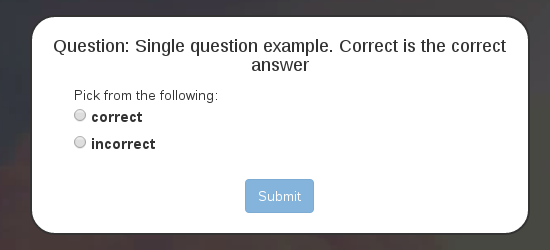
\includegraphics[width=\textwidth]{question_mockups/question-single.png}
	\caption{\label{Figure:Mockups_single} An example of a single answer question}
\end{figure}


\begin{figure}[h]
	\centering
		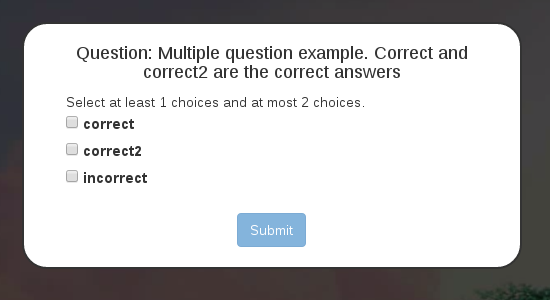
\includegraphics[width=\textwidth]{question_mockups/question-multiple.png}
	\caption{\label{Figure:Mockups_multiple} An example of a multiple answer question}
\end{figure}

\begin{figure}[h]
	\centering
		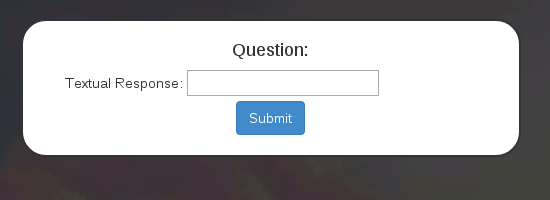
\includegraphics[width=\textwidth]{question_mockups/question-text.png}
	\caption{\label{Figure:Mockups_text} An example of a text type question}
\end{figure}

\begin{figure}[h]
	\centering
		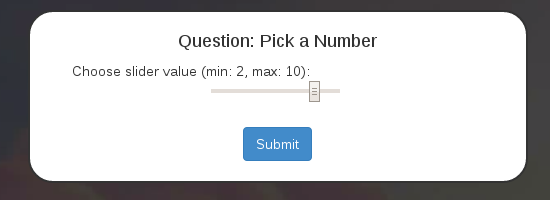
\includegraphics[width=\textwidth]{question_mockups/question-range.png}
	\caption{\label{Figure:Mockups_range} An example of a range type question}
\end{figure}

\begin{figure}[h]
	\centering
		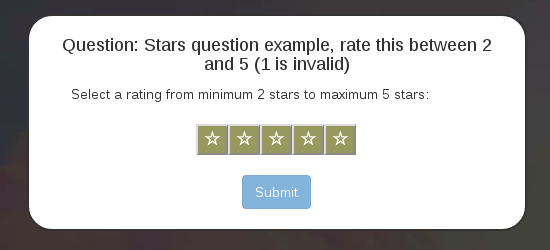
\includegraphics[width=\textwidth]{question_mockups/question-stars.png}
	\caption{\label{Figure:Mockups_stars} An example of a stars type question}
\end{figure}
